\chapter[Whole cell action potentials]{Action potentials: Summing up the effect of loads of ion channels}
\label{ap}

    In this final chapter we will use the theoretical drugs developed in various chapters above for whole cell simulations. So far we have studied very small parts of a cell. We started by studying the dynamics going on in a single dyad; see Figure \ref{cicr_1D}. The size of one dyad is
less than 1/1000 $\mu \mbox{m}^3$\cite{Bers2001} and we have been concerned with the concentration of calcium ions in this small volume. We have also studied the voltage dynamics in the vicinity of a single ion channel. The size of a single channel is about \GTLV{1 nm}. Now we address what is going on in a whole cell and it is important to realize that, compared to the single dyad and the single ion channel, the whole cell is huge; a normal ventricular cell is about 30,000 $\mu \mbox{m}^3$  \cite{Bers2001}, or on the order of  30 million times larger than the single dyad.

    In the analysis of single channels, we have regarded the state of a channel as a stochastic variable. In the whole cell, however, the effect of a huge number of channels is added and the sum can be modeled using deterministic equations. We will still use the same Markov model formalism in terms of reaction schemes to formulate the models, but now we will use the associated master equations (see page \pageref{master_equation}) to define the open probability of the channel. Thus we need to solve deterministic systems of ordinary differential equations to find the open probability as a function of time.

    Since the state of the channels will be represented using Markov model reaction schemes, we can study mutations in the same manner as we did for the single channel case. Therefore, we can use the results we derived above regarding optimal theoretical drugs for the single channel case for the whole cell case as well. The reasoning behind this was indicated earlier: If a mathematical model of a cell is constructed by using models of a huge number of single channels and we can repair the function of each single channel, the whole cell will be repaired.

    In this chapter we will start by introducing a model of the action potential of the whole cell. We will focus on a simplified model that will merely represent the action potential in a qualitatively relevant manner; it will not represent any particular action potential in a quantitatively correct manner.   Using numerical experiments, we will show that the model provides reasonable results for both wild type and various mutations. Finally, we will use the optimal theoretical drugs derived above and see that the effect of various mutations can be repaired using the theoretical drugs.

\section{Whole cell action potential model}
\label{sec:ap}


Our aim is now to introduce a reasonably simple action potential model for a whole cell. We will use the building blocks developed above and add some new features in order to get an action potential that is qualitatively reasonable.


\begin{figure}
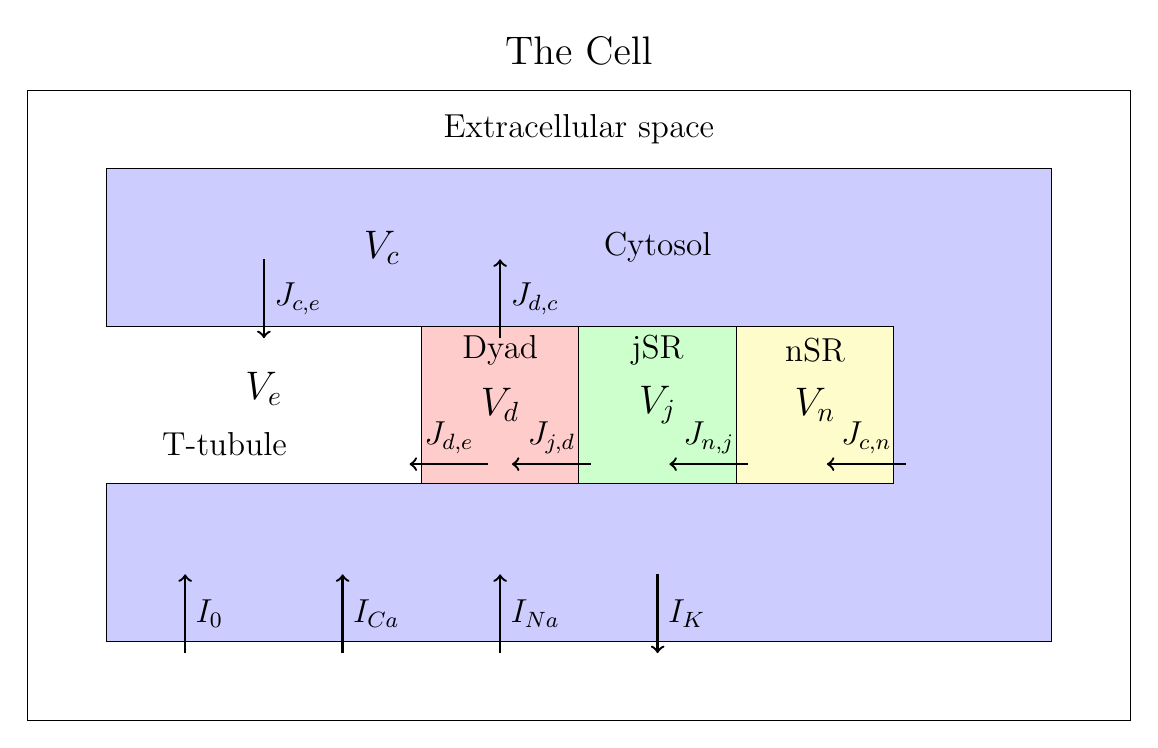
\begin{tikzpicture}[line width=0.3mm]
\tikzstyle{every node}=[font=\large]
\draw[line width=0,fill=white!80!white] (-1,-1) -- (13,-1) -- (13,7) -- (-1,7) -- (-1,-1);
\draw[line width=0,fill=white!80!blue] (0,0) -- (12,0) -- (12,6) -- (0,6)  -- (0,4) -- (10,4) -- (10,2) -- (0,2) -- (0,0);
\draw[line width=0,fill=white!80!yellow] (8,2) -- (10,2) -- (10,4) -- (8,4) -- (8,2);
\draw[line width=0,fill=white!80!green] (6,2) -- (8,2) -- (8,4) -- (6,4) -- (6,2);
\draw[line width=0,fill=white!80!red] (4,2) -- (6,2) -- (6,4) -- (4,4) -- (4,2);
\node[black!50!black] at (5, 3.0) {\Large{$V_{d}$}};
\node[black!50!black] at (7, 3.0) {\Large{$V_{j}$}};
\node[black!50!black] at (9, 3.0) {\Large{$V_{n}$}};
\node[black!50!black] at (5, 3.7) {Dyad};
\node[black!50!black] at (7, 3.7) {jSR};
\node[black!50!black] at (9, 3.7) {nSR};
\draw[->, black] (5,3.85) --node[right] {$J_{d,c}$} (5,4.85);
\draw[->, black] (2,4.85) --node[right] {$J_{c,e}$} (2,3.85);
\node[black!50!black] at (3.5, 5) {\Large{$V_{c}$}};
\node[black!50!black] at (2, 3.2) {\Large{$V_{e}$}};
\node[black!50!black] at (1.5, 2.5) {T-tubule};
\node[black!50!black] at (6, 6.5) {Extracellular space};
\node[black!50!black] at (7, 5) {Cytosol};
\node[black!50!black] at (6, 7.5) {\Large{The Cell}};
\draw[<-, black] (3.85,2.25) --node[above] {$J_{d,e}$} (4.85,2.25);
\draw[->, black] (6.15,2.25) --node[above] {$J_{j,d}$} (5.15,2.25);
\draw[->, black] (8.15,2.25) --node[above] {$J_{n,j}$} (7.15,2.25);
\draw[->, black] (10.15,2.25) --node[above] {$J_{c,n}$} (9.15,2.25);
\draw[->, black] (1,-0.15) --node[right] {$I_{0}$} (1,0.85);
\draw[->, black] (3,-0.15) --node[right] {$I_{Ca}$} (3,0.85);
\draw[->, black] (5,-0.15) --node[right] {$I_{Na}$} (5,0.85);
\draw[<-, black] (7,-0.15) --node[right] {$I_{K}$} (7,0.85);
%\draw[<->, black] (9,-0.15) --node[right] {$I_{NaK}$} (9,0.85);
\end{tikzpicture}
\caption{Sketch of the calcium dynamics and the fluxes and pumps involved. The volumes of the cytosol, the dyad, the junctional sarcoplasmic reticulum (JSR) and the network sarcoplasmic reticulum (NSR) are $V_c,\, V_d,\, V_j,$ and $V_n$, respectively.\label{fig:sketch}}
\end{figure}




The model consists of six main variables: $v, \, c_{e}, \, c_{c}, \, c_{d}, \, c_{j}$, and $c_{n}.$
Here $v,$ as usual, denotes the transmembrane potential given in mV. All the
other variables are concentrations given in $\mu$M; $c_{e}$ is the extracellular calcium concentration, $c_{c}$ is the cytosolic
concentration, $c_{d}$ is the concentration of the dyad, $c_{j}$ is the
concentration of the JSR, and finally $c_{n}$ is the concentration of the NSR;
see Figure \ref{fig:sketch}. In addition to these six main variables, we will have
variables associated with various Markov models; all these variables are between zero
and one; they also denote probabilities and they have no unit. The transmembrane
potential is governed by the equation
\begin{equation}
Cv^{\prime}=-\left(  I_{Na}+I_{Ca}+I_{K}+I_{0}\right)  \label{dvdt50}
\end{equation}
where the minus sign is according to convention in the field. Here $C$ denotes the
capacitance and is simply a constant that will be specified below. The current
$I_{0}$ represents a stimulus of the cell and we will use it below to initiate
action potentials. The sodium current $I_{Na},$ the calcium current $I_{Ca},$
and the potassium current $I_{K}$ need some attention and will be handled
separately.

\bigskip
In addition to the transmembrane potential, we need to keep track of
all five calcium concentrations.
%We will assume that the extracellular calcium concentration $c_{e}$ is given and that it is kept constant for all time; it will just enter as a paramter in the computations. But theconcentrations $c_{c},c_{d},c_{j}$ and $c_{n}$ must be updated dynamically.
By considering Figure \ref{fig:sketch}, we see that the cytosolic concentration can change in
three ways:\footnote{This is a major simplification; many other things can
happen to calcium but this rough description is sufficient for our purposes.
} (1) Calcium may diffuse into the cytosolic space from the
dyad,\footnote{It is important to recall here that when we talk about the dyad
now, we really refer to a space representing the sum of all the dyads of the
cell. So what used to be a very tiny place is not so tiny anymore.} leading to
an increase in the cytosolic concentrations; (2) it can be pumped from the cytosol into the
NSR and thereby reduce the cytosolic concentration; or, finally, (3) it can be
pumped out to the extracellular space, thereby reducing the cytosolic
concentration. The calcium concentration of the NSR, $c_{n},$ will be
increased as calcium is pumped into this space from the cytosol and reduced
by diffusion into its neighboring space, the JSR. In the JSR the calcium
concentration will increase through diffusion from the NSR and be reduced when
calcium is released through the ryanodine receptor (RyR) into the dyadic space. Finally, the
concentration in the dyad will increase when calcium is released from the JSR
to the dyad; it will be reduced as calcium diffuses out to the cytosol and
finally it will be increased when calcium is released into the dyad through
the L-type calcium channels (LCCs). In mathematical terms, we get the following system of
equations:
\begin{align}
V_{c}c_{c}^{\prime}  & =J_{d,c}-J_{c,n}-J_{c,e},\label{c51}\\
V_{n}c_{n}^{\prime}  & =J_{c,n}-J_{n,j},\label{c52}\\
V_{j}c_{j}^{\prime}  & =J_{n,j}-J_{j,d},\label{c53}\\
V_{d}c_{d}^{\prime}  & =J_{j,d}-J_{d,c}-J_{d,e}.\label{c54} \\
V_{e}c_{e}^{\prime}  & =J_{c,e}+J_{d,e}.\label{c55}
\end{align}
Here the notation $J_{x,y}$ denotes a flux of calcium from space $x$ to
space $y.$ So $J_{d,c}$ denotes the flux of calcium from the dyad ($d$) to
the cytosol ($c$) and, similarly, $J_{d,e}$ denotes the flux of calcium from
the  dyad ($d$)  to the extracellular ($e$) space. Here $V_{x}$ denotes the
volume fraction occupied by the space $x.$  The total amount of calcium in the system is given by
\begin{equation}
c=V_{c}c_{c}+V_{n}c_{n}+V_{j}c_{j}+V_{d}c_{d}+V_{e}c_{e}. \label{tot_ca}
\end{equation}



\subsection{Conservation of calcium}

%Suppose the cell membrane is completely closed so we have
%\begin{equation}
%J_{d,e}=J_{e,d}=0,
%\end{equation}
%then
It follows from the system (ref{c51})-(\ref{c55}) that
\begin{equation}
c^{\prime}=0,
\end{equation}
so the total amount of calcium is conserved no matter how the calcium
dynamics of the cell are organized.

%This observation motivates a modeling
%requirement for the fluxes across the cell membrane. We are modeling a
%process where the cell is supposed to be stimulated by a current, then undergo
%an action potential of length $T$, and then turn back to a normal resting
%state and wait for another stimulus.
%In general, we have
%\begin{equation}
%c^{\prime}=J_{e,d}-J_{d,e}
%\end{equation}
%and in order for the total calcium concentration to return to the same value
%after an action potential, we need to have
%\begin{equation}
%c(T)=c(0)
%\end{equation}
%\bigskip and this is satisfied if
%\begin{equation}
%\int_{0}^{T}J_{e,d}dt=\int_{0}^{T}J_{d,e}dt.\label{J_req}
%\end{equation}
%Below, we will make sure that we tune our parameters such that this requirement (at least approximately) is satisfied.


\subsection{Definition of calcium-related fluxes}

\begin{table}
\begin{center}
\begin{tabular}{|c|c|} \hline
$V_d$ & 0.1\% \\ \hline
$V_j$ & 0.3\% \\ \hline
$V_n$ & 1\% \\ \hline
$V_c$ & 98.6\% \\ \hline
\end{tabular}
\caption{The table shows the relative size of the intracellular spaces. Note that the volume fractions
of the intracellular space add up to $100\%$. In addition, $V_e$ represents $100\%$ of the extracellular space.
We assume that both the extracellular space and the total intracellular space are 30.4 pL
%The extracellular space is 30.4 pL and we assume that it equals the total intracellular space.
}
\end{center}
\end{table}

\begin{table}
\begin{center}
\begin{tabular}{|c|c|} \hline
$k_{c,n}$ & 0.01 \\ \hline
$k_{j,d}$ & 0.01 \\ \hline
$k_{d,c}$ & 0.001 \\ \hline
$k_{d,e}$ & 0.0001 \\ \hline
$k_{n,j}$ & 0.0001  \\ \hline
$k_{c,e}$ & 0.00001 \\ \hline
\end{tabular}
\caption{\label{tab:k}Constants used to define the fluxes between the different spaces. The constants are in units of 1/ms.
}
\end{center}
\end{table}

\begin{figure}[ptb]
\begin{center}
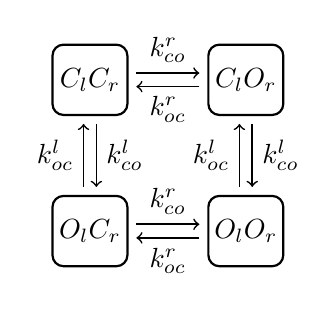
\begin{tikzpicture}[
   font=\sffamily,
   every matrix/.style={ampersand replacement=\&,column sep=1cm,row sep=1cm},
   state/.style={draw,thick,rounded corners,inner sep=.3cm},
   to/.style={->,semithick,shorten >=0.1cm,shorten <=0.1cm},
   Q/.style={->,semithick,sloped,pos=0.700000,shorten >=0.1cm,shorten <=0.1cm},
   every node/.style={auto}]
\matrix{
\node[state] (C_{l}C_{r}) {\parbox{10pt}{\centerline{$C_{l}C_{r}$}}};\&\node[state] (C_{l}O_{r}) {\parbox{10pt}{\centerline{$C_{l}O_{r}$}}};\\
\node[state] (O_{l}C_{r}) {\parbox{10pt}{\centerline{$O_{l}C_{r}$}}};\&\node[state] (O_{l}O_{r}) {\parbox{10pt}{\centerline{$O_{l}O_{r}$}}};\\
};
\draw[to]  (C_{l}C_{r}.10) to node {$k_{co}^{r}$} (C_{l}O_{r}.170);
\draw[to]  (C_{l}C_{r}.280) to node {$k_{co}^{l}$} (O_{l}C_{r}.80);
\draw[to]  (C_{l}O_{r}.190) to node {$k_{oc}^{r}$} (C_{l}C_{r}.350);
\draw[to]  (C_{l}O_{r}.280) to node {$k_{co}^{l}$} (O_{l}O_{r}.80);
\draw[to]  (O_{l}C_{r}.100) to node {$k_{oc}^{l}$} (C_{l}C_{r}.260);
\draw[to]  (O_{l}C_{r}.10) to node {$k_{co}^{r}$} (O_{l}O_{r}.170);
\draw[to]  (O_{l}O_{r}.100) to node {$k_{oc}^{l}$} (C_{l}O_{r}.260);
\draw[to]  (O_{l}O_{r}.190) to node {$k_{oc}^{r}$} (O_{l}C_{r}.350);
\end{tikzpicture}
\end{center}
\caption{Markov model including four possible states: $C_{l}C_{r}$ (both
closed), $C_{l}O_{r}$ (LCC closed, RyR open), $O_{l}O_{r}$ (both open), and
$O_{l}C_{r}$ (LCC open, RyR closed).}
\label{eq:m_rl2}
\end{figure}

%The states of this combined Markov model are given by $C_{l}C_{r}$ (both
%closed), $C_{l}O_{r}$ (LCC closed, RyR open), $O_{l}O_{r}$ (both open), and
%$O_{l}C_{r}$ (LCC open, RyR closed). In our computations, we use the rates shown in Table \ref{fundtions2}.

%following functions
%\begin{equation}
\begin{table}
\begin{center}
%\begin{tabular}[c]{|l|l|l|l|} \hline
%$k_{co}^{r}=\mu \frac{x^4}{K(y)^4+x^4}$ & $k_{oc}^{r}=1$ &
%$K(y) =  K_{max}-y/1000$ & $K_{max} = 7.4\mu$M \\ \hline
%$k_{co}^{l}=\eta\, l_{\infty}(V)/\tau_l$ & $k_{oc}^{l}=(1-l_{\infty}(V))/\tau_l%$ &$l_{\infty}(V) = 0.01 \exp(-(V-5)^2/500)$
%&$\tau_l=1$ms \\ \hline
\begin{tabular}[c]{|l|l|} \hline
RyR: & LCC: \\
$k_{co}^{r}(c_d,c_j)=\mu \frac{c_d^4}{K(c_j)^4+c_d^4} \text{ ms}^{-1}$ &$k_{co}^{l}(v)=\eta\, l_{\infty}(v)/\tau_l$ \\
$k_{oc}^{r}=1 \text{ ms}^{-1}$ & $k_{oc}^{l}(v)=(1-l_{\infty}(v))/\tau_l$ \\
$K(c_j) = 20+1000(\frac{1000-c_j}{600})^2$ &  $ l_{\infty}(v) = \exp(-(\frac{v-55}{10})^2)$ \\
 & $\tau_l=1$ ms\\ \hline
\end{tabular}
\end{center}
%\end{equation}
\caption{Reaction rates used in the Markov model illustrated in
Figure \ref{eq:m_rl2}.
As usual,  $\mu \ge 1$ denotes the mutation severity
index of the RyR and $\eta \ge 1$ denotes the mutation severity
index of the LCC. }
\label{functions2}
\end{table}

We need to define all the fluxes entering the system (ref{c51})-(\ref{c55}) and we start with the simple diffusion fluxes. Some of
them have been used in earlier chapters, but we need a little more notation
here, so we redefine all the terms.

\subsubsection{Flux $J_{d,c}$ from the dyad to the cytosol}
We assume that the pure diffusion flux
from the dyad to the cytosol can be written as
\begin{equation}
J_{d,c}=k_{d,c}\left(  c_{d}-c_{c}\right).
 \label{J_dc}
\end{equation}
Here we assume that $k_{d,c}$ is a constant and the value used in our computations is given in Table \ref{tab:k}.

\subsubsection{Flux $J_{n,j}$ from the NSR to the JSR}
Similarly, we assume that the diffusion flux from the NSR to the JSR can be written as
\begin{equation}
J_{n,j}=k_{n,j}\left(  c_{n}-c_{j}\right), \label{J_nj}
\end{equation}
where $k_{n,j}$ is assumed to be a constant (see Table \ref{tab:k}).

\subsubsection{RyR flux $J_{j,d}$ from the JSR to the dyad}
The
flux from the JSR to the dyad can be written in the form
\begin{equation}
J_{j,d}=o_{j,d}k_{j,d}\left(  c_{j}-c_{d}\right), \label{J_jd}
\end{equation}
where, as usual, $o_{j,d}$ is governed by a Markov model and $k_{j,d}$ is a
constant giving the speed of diffusion when the RyR channel (situated between
the JSR and the dyad) is open.

The variable $o_{j,d}$ is governed by the Markov model
used in Chapter \ref{cicr}. For convenience the Markov model is repeated here in Figure \ref{eq:m_rl2} and  the functions
used in the model are given in Table \ref{functions2}. Note that $o_{j,d}$ is the probability of being in the state $C_lO_r$ or the state $O_lO_r$ of the Markov model given in Figure \ref{eq:m_rl2}.

%The parameters and functions are unaltered, except for $K(y)$
%the halv-saturation constant
%which has been changed to:
%\begin{equation}
%K(y) = 20+1000(\frac{1000-y}{600})^2. \label{halfmax}
%\end{equation}

%have been adapted to the current setting:
%illustrated in Figure xxx and the associated system of ordinary differential equations are given by xxx:
%\textbf{GTL: Insert the Markov model (ode-system and Figure) that you actually use.}



\subsubsection{Flux from the extracellular space to the dyad: $J_{d,e}$}

 This flux was introduced above (see page \pageref{GHK}) and referred to as the Goldman-Hodgkin-Katz (GHK) flux. In the present notation, we write

\begin{equation}
J_{d,e}=o_{d,e} k_{d,e} \frac{c_d-c_{e}e^{-\frac{v}{v_0}}}{1-e^{-\frac{v}{v_0}}}\frac{v}{v_0}.\label{J_ed}
\end{equation}
\graytable{l}{
{|c|c|} \hline
$F$ & $96485.3$ C mol$^{-1}$\\ \hline
$R$ & $8.3145$ J mol$^{-1}$K$^{-1}$\\\hline
$T$ & 310 K\\\hline
$v_0$ & 13.357 mV\\ \hline
}{Parameters in (\ref{J_ed}).\label{FRT_ed}}
Here %$D$ is Fick's diffusion constant,
$F$ is Faraday's constant, $R$ is the gas constant,
and $T$ is the absolute temperature and we have defined
\[
v_0=\frac{RT}{2F}.
\]
 The parameters involved in defining the $J_{d,e}$ flux are given in Table \ref{FRT_ed}. Furthermore, $o_{d,e}$ is governed by the Markov model
 given in Figure \ref{eq:m_rl2}. Here $o_{d,e}$ is the probability of being in the state $O_lC_r$ or the state $O_lO_r$ of the Markov model
  in Figure \ref{eq:m_rl2}.




%\[ l_{\infty}(v) = \exp(-(\frac{v-55}{10})^2). \]
%}
%presented in Figure xxx. The associated system of ordinary differential equations is given by xxxGTLxxx.
%xxx. \textbf{GTL: Insert the LCC model (ode-system and Figure) that you
%actually use (I do not if you want to couple the two models or treat them
%separately (LCC and RYR).}




\subsection{Definition of calcium pumps}


The terms $J_{c,e}$ and $J_{c,n}$ remain to be defined. These terms are active
fluxes, or pumps, that continuously remove calcium from the cytosol
and out to the extracellular domain $(J_{c,e})$ and into the NSR $(J_{c,n}).$
These pumps transport calcium against a considerable concentration gradient and
the operation therefore requires energy. In our model we do not track the
energy consumption and we simply introduce the pumps:
\begin{equation}
J_{c,e}=k_{c,e} (c_c-c_e/18000)  \label{J_ce}
\end{equation}
and
\begin{equation}
J_{c,n}= k_{c,n} (c_c-c_n/10000).  \label{J_cn}
\end{equation}


%xxx \textbf{GTL: insert the pumps you are using (follow the notational convention).}

\subsection{Definition of the currents}

The currents $I_{Na},\, I_K$ and $I_{Ca}$ of (\ref{dvdt50}) remain to be defined. Each current will be written in the form
\[
I_x=o_x g_x (v-v_x),
\]
where  $o_x$ is the open probability of the channel given by the continuous version of a Markov model, $g_x$ is the maximum conductance of the channel, and $v_x$ is the resting potential.

\subsubsection{Sodium current $I_{Na}$}

The sodium current has been studied above; see Chapters \ref{simple_Na} and \ref{burst_chap}. The model takes the form
\begin{equation}
I_{Na}= o_{Na} g_{Na}(v-v_{Na}),   \label{J_Na}
\end{equation}
where the open probability $o_{Na}$ is the sum of the probability of being in the $O$ or the $O^*$ state of the Markov model of Figure  \ref{wtreac3300}.

\begin{figure}[ptb]
\begin{center}
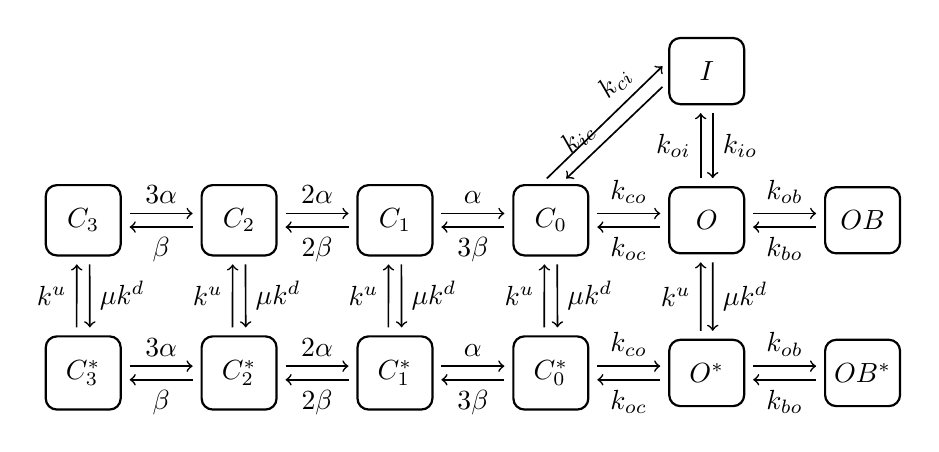
\begin{tikzpicture}[
   font=\sffamily,
   every matrix/.style={ampersand replacement=\&,column sep=1cm,row sep=1cm},
   state/.style={draw,thick,rounded corners,inner sep=.3cm},
   to/.style={->,semithick,shorten >=0.1cm,shorten <=0.1cm},
   Q/.style={->,semithick,sloped,pos=0.700000,shorten >=0.1cm,shorten <=0.1cm},
   every node/.style={auto}]
\matrix{
\&\&\&\&\node[state] (I) {\parbox{10pt}{\centerline{$I$}}};\&\\
\node[state] (C_{3}) {\parbox{10pt}{\centerline{$C_{3}$}}};\&\node[state] (C_{2}) {\parbox{10pt}{\centerline{$C_{2}$}}};\&\node[state] (C_{1}) {\parbox{10pt}{\centerline{$C_{1}$}}};\&\node[state] (C_{0}) {\parbox{10pt}{\centerline{$C_{0}$}}};\&\node[state] (O) {\parbox{10pt}{\centerline{$O$}}};\&\node[state] (OB) {\parbox{10pt}{\centerline{$OB$}}};\\
\node[state] (C_{3}^{*}) {\parbox{10pt}{\centerline{$C_{3}^{*}$}}};\&\node[state] (C_{2}^{*}) {\parbox{10pt}{\centerline{$C_{2}^{*}$}}};\&\node[state] (C_{1}^{*}) {\parbox{10pt}{\centerline{$C_{1}^{*}$}}};\&\node[state] (C_{0}^{*}) {\parbox{10pt}{\centerline{$C_{0}^{*}$}}};\&\node[state] (O^{*}) {\parbox{10pt}{\centerline{$O^{*}$}}};\&\node[state] (OB^{*}) {\parbox{10pt}{\centerline{$OB^{*}$}}};\\
};
\draw[to]  (O^{*}.100) to node {$k^{u}$} (O.260);
\draw[to]  (O^{*}.10) to node {$k_{ob}$} (OB^{*}.170);
\draw[to]  (O^{*}.190) to node {$k_{oc}$} (C_{0}^{*}.350);
\draw[to]  (O.280) to node {$\mu k^{d}$} (O^{*}.80);
\draw[to]  (O.100) to node {$k_{oi}$} (I.260);
\draw[to]  (O.190) to node {$k_{oc}$} (C_{0}.350);
\draw[to]  (O.10) to node {$k_{ob}$} (OB.170);
\draw[to]  (I.280) to node {$k_{io}$} (O.80);
\draw[Q]  (I.195) to node {$k_{ic}$} (C_{0}.75);
\draw[to]  (C_{0}.10) to node {$k_{co}$} (O.170);
\draw[Q]  (C_{0}.105) to node {$k_{ci}$} (I.165);
\draw[to]  (C_{0}.190) to node {$3\beta$} (C_{1}.350);
\draw[to]  (C_{0}.280) to node {$\mu k^{d}$} (C_{0}^{*}.80);
\draw[to]  (C_{1}.10) to node {$\alpha$} (C_{0}.170);
\draw[to]  (C_{1}.190) to node {$2\beta$} (C_{2}.350);
\draw[to]  (C_{1}.280) to node {$\mu k^{d}$} (C_{1}^{*}.80);
\draw[to]  (C_{2}.10) to node {$2\alpha$} (C_{1}.170);
\draw[to]  (C_{2}.190) to node {$\beta$} (C_{3}.350);
\draw[to]  (C_{2}.280) to node {$\mu k^{d}$} (C_{2}^{*}.80);
\draw[to]  (C_{3}.10) to node {$3\alpha$} (C_{2}.170);
\draw[to]  (C_{3}.280) to node {$\mu k^{d}$} (C_{3}^{*}.80);
\draw[to]  (OB.190) to node {$k_{bo}$} (O.350);
\draw[to]  (OB^{*}.190) to node {$k_{bo}$} (O^{*}.350);
\draw[to]  (C_{0}^{*}.10) to node {$k_{co}$} (O^{*}.170);
\draw[to]  (C_{0}^{*}.100) to node {$k^{u}$} (C_{0}.260);
\draw[to]  (C_{0}^{*}.190) to node {$3\beta$} (C_{1}^{*}.350);
\draw[to]  (C_{1}^{*}.100) to node {$k^{u}$} (C_{1}.260);
\draw[to]  (C_{1}^{*}.10) to node {$\alpha$} (C_{0}^{*}.170);
\draw[to]  (C_{1}^{*}.190) to node {$2\beta$} (C_{2}^{*}.350);
\draw[to]  (C_{2}^{*}.100) to node {$k^{u}$} (C_{2}.260);
\draw[to]  (C_{2}^{*}.10) to node {$2\alpha$} (C_{1}^{*}.170);
\draw[to]  (C_{2}^{*}.190) to node {$\beta$} (C_{3}^{*}.350);
\draw[to]  (C_{3}^{*}.100) to node {$k^{u}$} (C_{3}.260);
\draw[to]  (C_{3}^{*}.10) to node {$3\alpha$} (C_{2}^{*}.170);
\end{tikzpicture}
\end{center}
\caption{This figure is a copy of Figure \ref{burstdrg} and it illustrates a Markov model of the mutant sodium channel.
 The model consists of the states $O,I,OB,C_{0}
,C_{1},C_{2},$ and $C_{3}$ of the normal mode and $OB^*,O^{*},C^{*}_{0},C^{*}
_{1},C^{*}_{2},$ and $C^{*}_{3}$ of the burst mode (lower part). }
\label{wtreac3300}
\end{figure}

\subsubsection{Potassium current $I_{K}$}

The potassium current is written in the form
\begin{equation}
I_{K}= (o_{K} g_{K}(v) + g_{K1}(v)) (v-v_{K}),   \label{J_K}
\end{equation}
where the open probability $o_{K}$ is given by the Markov model of Figure  \ref{K1} with rates
\begin{align*}
\alpha(v) &  = e^{-7+0.03v},\\
\beta(v) &  = e^{-8-0.03v}. \\
\end{align*}
The voltage-dependent conductances are given by
\begin{align*}
g_K(v) &=  0.1 e^{-0.03v}, \\
g_{K1}(v) &= \frac{1}{1+e^{0.1 v+10}}. \\
\end{align*}


\begin{figure}[ptb]
\begin{center}
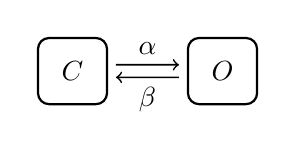
\begin{tikzpicture}[
   font=\sffamily,
   every matrix/.style={ampersand replacement=\&,column sep=1cm,row sep=1cm},
   state/.style={draw,thick,rounded corners,inner sep=.3cm},
   to/.style={->,semithick,shorten >=0.1cm,shorten <=0.1cm},
   Q/.style={->,semithick,sloped,pos=0.700000,shorten >=0.1cm,shorten <=0.1cm},
   every node/.style={auto}]
\matrix{
\node[state] (C) {$C$};\&\node[state] (O) {$O$};\\
};
\draw[to]  (O.190) to node {$\beta$} (C.350);
\draw[to]  (C.10) to node {$\alpha$} (O.170);
\end{tikzpicture}
\end{center}
\caption{Markov model of a potassium channel
consisting of one closed and one open state. }
\label{K1}
\end{figure}


\subsubsection{Calcium current $I_{Ca}$}

The calcium current is given by the calcium flux  $J_{d,e}$ from the dyad to the extracellular space plus the flux $J_{c,e}$ from the cytosol to the extracellular space.
In order to use these fluxes  in the equation governing the transmembrane potential, we need convert to current density,
\begin{equation}
I_{Ca}= 2 F\frac{V}{A} (-J_{d,e}-J_{c,e}).   \label{I_Ca}
\end{equation}
Here $V=30.4$ pL is the cell volume and $A=1.4\cdot 10^{-4} \text{ cm}^2$ is the cell area.

\subsection[Markov models as ODEs]{Markov models in terms of systems of differential equations}

The model of the action potential for a whole cell is a system of ordinary differential equations. For parts of the system this is clear from the equations,
but for the Markov models, this may seem unclear. In Section \ref{me_eq} we explained how to formulate a system of ordinary differential equation associated with the reaction scheme defining a Markov model.  Since the Markov models considered in the present chapter are considerably more complex, we will give one more example of this transition in order to clarify matters. To this end, consider the Markov model presented in Figure \ref{wtreac3331}.
 The associated system of ordinary differential equations governing the probabilities is given by
\begin{align*}
o^{\prime}  & =k_{io}i+k_{co}c_{0}-\left(  k_{oc}+k_{oi}\right)  o,\\
i^{\prime}  & =k_{oi}o+k_{ci}c_{0}-\left(  k_{io}+k_{ic}\right)  i,\\
c_{0}^{\prime}  & =k_{oc}o+k_{ic}i+\alpha c_{1}-\left(  k_{co}+k_{ci}
+3\beta\right)  c_{0},\\
c_{1}^{\prime}  & =3\beta c_{0}+2\alpha c_{2}-\left(  2\beta+\alpha\right)
c_{1},\\
c_{2}^{\prime}  & =2\beta c_{1}+3\alpha c_{3}-\left(  2\alpha+\beta\right)
c_{2},\\
c_{3}^{\prime}  & =\beta c_{2}-3\alpha c_{3}.
\end{align*}
Here, $o$ denotes the open probability of the sodium channel,  $c_0$ is the probability of the $C_0$ state, and so forth. Ideally, we would write $o_{Na}$ for $o$, $c_{0,Na}$ for $c_0$, and so forth, but it becomes clumsy. Since these variables represent probabilities, they sum to one (for all time) and we can therefore reduce the number of unknowns in the system by one.

Based on this example, it should be straightforward to formulate the system of ordinary differential equations associated with the more complex Markov model given in Figure \ref{wtreac3300}.

\begin{figure}[ptb]
\begin{center}
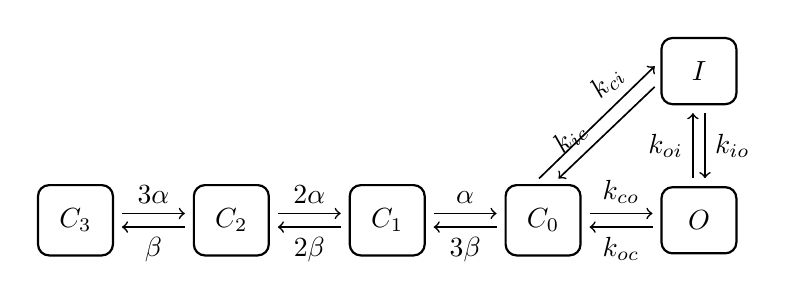
\begin{tikzpicture}[
   font=\sffamily,
   every matrix/.style={ampersand replacement=\&,column sep=1cm,row sep=1cm},
   state/.style={draw,thick,rounded corners,inner sep=.3cm},
   to/.style={->,semithick,shorten >=0.1cm,shorten <=0.1cm},
   Q/.style={->,semithick,sloped,pos=0.700000,shorten >=0.1cm,shorten <=0.1cm},
   every node/.style={auto}]
\matrix{
\&\&\&\&\node[state] (I) {\parbox{10pt}{\centerline{$I$}}};\\
\node[state] (C_{3}) {\parbox{10pt}{\centerline{$C_{3}$}}};\&\node[state] (C_{2}) {\parbox{10pt}{\centerline{$C_{2}$}}};\&\node[state] (C_{1}) {\parbox{10pt}{\centerline{$C_{1}$}}};\&\node[state] (C_{0}) {\parbox{10pt}{\centerline{$C_{0}$}}};\&\node[state] (O) {\parbox{10pt}{\centerline{$O$}}};\\
};
\draw[to]  (O.100) to node {$k_{oi}$} (I.260);
\draw[to]  (O.190) to node {$k_{oc}$} (C_{0}.350);
\draw[to]  (I.280) to node {$k_{io}$} (O.80);
\draw[Q]  (I.195) to node {$k_{ic}$} (C_{0}.75);
\draw[to]  (C_{0}.10) to node {$k_{co}$} (O.170);
\draw[Q]  (C_{0}.105) to node {$k_{ci}$} (I.165);
\draw[to]  (C_{0}.190) to node {$3\beta$} (C_{1}.350);
\draw[to]  (C_{1}.10) to node {$\alpha$} (C_{0}.170);
\draw[to]  (C_{1}.190) to node {$2\beta$} (C_{2}.350);
\draw[to]  (C_{2}.10) to node {$2\alpha$} (C_{1}.170);
\draw[to]  (C_{2}.190) to node {$\beta$} (C_{3}.350);
\draw[to]  (C_{3}.10) to node {$3\alpha$} (C_{2}.170);
\end{tikzpicture}
\end{center}
\caption{Markov model of a wild type sodium channel consisting of an open
state $(O)$, an inactivated state $(I)$, and four closed states $(C_{0}
,C_{1},C_{2}, \text{ and }C_{3})$. }
\label{wtreac3331}
\end{figure}


\section[Numerical action potential; wild type]{Numerical simulations using the action potential model for wild type Markov models}

The complete version of the model presented above can be written in the compact form
\begin{align}
Cv^{\prime}  & =-\left(  I_{Na}+I_{Ca}+I_{K}+I_{0}\right),  \label{s401}\\
u^{\prime}  & =F(v,u)\label{s402},
\end{align}
where $v$ is the transmembrane potential and all other variables are gathered in the vector $u$. The initial conditions used in the simulations are given in Table \ref{tab:init}. In addition, we need to specify the applied current $I_0$. This current will be zero most of the time, but it will be turned on every 500 ms in order to mimic periodic stimulation of the cell. More specifically,
we hold $I_0$ = -6 mV/ms for 5 ms at the start of each cycle.

\begin{table}
\begin{center}
\begin{tabular}{|c|c|} \hline
$v$ & -85 mV \\ \hline
$c_{d}$ & 0.1 $\mu$M \\ \hline
$c_{c}$ & 0.1 $\mu$M \\ \hline
$c_{j}$ & 1000 $\mu$M \\ \hline
$c_{n}$ & 1000 $\mu$M \\ \hline
$c_{e}$ & 1800 $\mu$M \\ \hline
\end{tabular}
\caption{Initial conditions. The Markov models for the LCC and RyR were initially set to closed and the Markov model for sodium channel was set to be in the state $C_3$. Starting with these conditions, the code is run for 1000 cycles in order to generate the initial conditions used in generating the figures below. The exact numbers obtained depend upon the chosen cycle length. \label{tab:init}}
\end{center}
\end{table}





\subsection{Single action potential}

In Figure \ref{ap:single1} we show the transmembrane potential and all the calcium concentration for a single action potential. There are a number of interesting effects acting together to generate the action potential. Let us consider some of them in some detail.

FIGURE: [fig/ap_single1.pdf, width=500 frac=0.8] The action potential of the model described in the present chapter. The membrane potential (upper left) and the dynamics of the five calcium concentrations are shown for 500 ms. The action potential is initiated by holding $I_0$ = -6 mV/ms for 5 ms. All variables return to their resting values after about 500 ms.  label{ap:single1}

FIGURE: [fig/ap_single2.pdf, width=500 frac=0.8] The first 20 ms of the simulation shown in Figure \ref{ap:single1}. Note the log scale in the upper right panel. There we see a slow rise due to the LCC opening, followed by a fast rise due to the RyR opening. label{ap:single2}

In Figure \ref{ap:single2} we show the first 20 ms of the computation. In the left panel we show the transmembrane potential $v$ (upper left panel), the open probability $o_{Na}$ (middle left panel), and the sodium current $I_{Na}$ (lower left panel). Observe that when the cell is stimulated by the applied current $I_0$, the transmembrane potential increases. This increase leads to an increased open probability of the sodium channel. When the sodium channel opens, the sodium current becomes large (or very negative, to be precise), which leads to a fast increase of the transmembrane potential. As the transmembrane potential reaches its peak value (at about 15 ms), the open probability starts to decline, since the channel inactivates. In the three right panels, we show the calcium concentration of the dyad $c_d$ (upper right panel), the calcium flux $J_{d,e}$ (middle right panel), and the open probability of the RyR channel  (lower right panel). We see that when the transmembrane potential starts increasing, the calcium flux $J_{d,e}$ increases and the calcium concentration of the dyad increases. This increase leads to the increased open probability (lower right panel) of the RyR channel and therefore the dyad concentration increases rapidly.

In Figure \ref{ap:single3}, we show the return to the stable equilibrium solution. In the left panel, we show the transmembrane (upper left panel), the open probability of the LCC (middle left panel), and the open probability of the gated potassium channel. After the sodium channel has switched off (see Figure \ref{ap:single2}), the calcium current contributes to a continued depolarized state. However, after about 20 ms the transmembrane potential starts declining because of a substantial (positive) potassium current.
%the open probability $o_{Na}$ (middle left panel), and the potassium current $I_K$ (lower left panel). We see that the sodium channel now is not conducting since $o_{Na}$ is almost zero. The transmembrane potential is reduced and this is due to a substantial (positive) potassium current.

In the right panels, we follow the development of the calcium concentration of the dyad $c_d$ (upper right panel),  the calcium concentration
\GTLV{$c_j$ of the JSR},
%$c_n$ of the NSR
(middle right panel), and the open probability of the RyR channel, denoted $o_{j,d}$ (lower right panel).
%\GTLV{we see that the jSR consentration falls rapidly when channel is open. This causes the channel to close, due an incrase in the half-maximum  constant (see
%$equation \ref{halfmax})}.
%We see that the dyad concentration is reduced and that the RyR is practically closed. The increase of the calcium concentration in the NSR is due to the pump $J_{c,n}$ and to the fact that the RyR channel is closed.

FIGURE: [fig/ap_single3.pdf, width=500 frac=0.8] After about 15 ms, the transmembrane potential (upper left) reaches its peak value and enters the plateau phase before it starts to decline toward the stable equilibrium solution.  label{ap:single3}

\subsection{Many action potentials}

In Figure \ref{ap:multiple}, we show the action potential for a simulation running for 25,000 ms. The left panel shows the transmembrane potential $v$ (upper left panel), the calcium concentration $c_d$ of the dyad (middle left panel), and the extracellular calcium concentration $c_e$ (lower left panel). From top to bottom in the right panels, we show the cytosolic calcium concentration $c_c$, the NSR calcium concentration $c_n$, and finally the JSR calcium concentration $c_j$. All variables return to their initial values and the rhythm seems to be perfect.
%In Figure xxx5, we show exactly the same variables after 10000 action potentials and it looks exactly the same.

FIGURE: [fig/ap_multiple.pdf, width=500 frac=0.8] The action potential running for 25,000 ms (50 beats). All variables return to their equilibrium values before a new action potential is initiated (every 500 ms).  label{ap:multiple}

\section[Changing the mean open time]{Changing the mean open time of the sodium channel while keeping the equilibrium probability fixed changes the action potential}
\label{sec:ap_mot}

We consider a case where we multiply all rates of the Markov model (see Figure \ref{wtreac3300}) of the sodium channel by the same factor. Here we use the wild type case ($\mu=1$) and the drug parameters ($k_{ob}, k_{bo}$) are set to zero. This will change the mean open time, but not the equilibrium probabilities. The results are given in Figure \ref{ap:mot}, where the blue line illustrates the results using default parameters, the red line represents the solution when all the rates are multiplied by 1.3, and finally the green line represents the solution when all the rates are multiplied by 0.7. We observe that the action potential changes substantially when the rates are changed (and the mean open time is changed), even though the equilibrium probabilities are kept unchanged.

FIGURE: [fig/ap_mot.pdf, width=500 frac=0.8] Slower dynamics (green) lead to later inactivation, yielding a higher plateau. Quicker dynamics (red) lead to faster recovery from inactivation, allowing a stronger late current.  label{ap:mot}


\section[Numerical action potential; mutations]{Numerical simulations using the action potential model when the cell is affected by a mutation}

We will use the model of the action potential for the whole cell introduced above to study the effect of mutations. We have studied many different theoretical models of mutations earlier, but here we will limit ourselves to study the effect of one theoretical model of a sodium channel mutation, one model of a RyR mutation, and one model of an LCC mutation. We will also see how the theoretical drugs derived above handle these mutations.




\subsection{Mutation of the sodium channel}

We consider a mutation of the sodium channel of the form presented in Figure \ref{wtreac3300}.
In Figure \ref{ap:burst_mut} we show simulation results comparing the wild type ($\mu=1$, blue),
the mutant ($\mu=10$, green), and a simulation (red) where  a drug is applied to the mutant case.
The Markov model describing the open state drug is given
in Figure \ref{wtreac3300}, where we have used drug parameters given by
\[
k_{bo} = k_{io}, \mbox{\ and \ }
k_{ob}=\left(  \mu-1\right)  \frac{k^{d}k^{u}k_{oi}}{\left(  k^{u}+\mu
k^{d}\right)  \left(  k^{u}+k^{d}\right)  };
\]
see (\ref{na_drug_ob}) and (\ref{na_drug_bo}).
As in the single channel case, we observe that the theoretical drug is able to repair the effect of the mutation.


FIGURE: [fig/ap_burst_mut.pdf, width=500 frac=0.8] The figure shows the action potential of the wild type (blue), the mutant (green), and the
mutant after the application of the drug (red). label{ap:burst_mut}

\subsection{Mutation of the RyR}

In Figure \ref{ap:ryr_mut} we have simulated mutation in the RyR using the Markov model given in Figure \ref{eq:m_rl2}. The figure shows the
wild type (blue, $\mu=1$), the mutant (green, $\mu=3$), and the mutant where the drug has been applied (red). We have used a closed state drug  computed as described in (\ref{closed_drg}) and (\ref{optimal_closed_charac}) and we observe that the theoretical drug is able to repair the effect of the mutation.
%{\bf xxxGTL: Is this a RyR mutation?  If RYR- what is the Markov model with drugs? Refs to model}






FIGURE: [fig/ap_ryr_mut.pdf, width=500 frac=0.8] The cytosolic calcium concentration for wild type (blue, $\mu=1$), the mutant (green, $\mu=3$), and the mutant after the application of the drug (red). We have used a closed state drug  as defined in (\ref{closed_drg}) with $k_{bc}=0.5$ ms$^{-1}$ and $k_{cb}=(\mu-1)k_{bc}$; see (\ref{optimal_closed_charac}).  label{ap:ryr_mut}

\subsection{Mutation of the LCC}

In Figure \ref{ap:lcc_mut} we have simulated mutation in the LCC channel, using $\eta=3$.
%{\bf xxxGTL: Is this a LCC mutation?  If LCC- what is the Markov model with drugs? Refs to model}
We model the mutation and the drug as defined in (\ref{closed_drg}) and (\ref{optimal_closed_charac}). As usual, $k_{bc}$ is a free parameter that must be chosen sufficiently large. Again, we note that the theoretical drug repairs the effect of the mutation.

FIGURE: [fig/ap_lcc_mut.pdf, width=500 frac=0.8] LCC mutation. The cytosolic calcium concentration for the wild type (blue, $\eta=1$), the mutant (green $\eta=3$), and the mutant case where the theoretical drug is applied (red). In the computations we have used $k_{bc}=0.05$ ms$^{-1}$; for larger values of $k_{bc}$ the results overlap with the wild type case. label{ap:lcc_mut}


\section{Notes}

\begin{enumerate}
\item The action potential model discussed in Section \ref{sec:ap} and used throughout this chapter is only of qualitative relevance; no effort is made to mimic the properties of one particular cell. The field of models for the action potential is huge and growing. A great collection of models is provided by the Auckland Bioengineering Institute at the University of Auckland and their collaborators; see CellML.org. Recent models tend to be increasingly complex and hard to deal with from a mathematical perspective, but clearly the models become more and more realistic in terms of mimicking the properties of the actual action potential.  As mentioned earlier, there are comprehensive introductions to the cardiac action potential, such as Rudy \cite{Rudy2012} and Rudy and Silva \cite{Rudy2006}.
\item In these notes we have used Matlab as the computational platform for all our simulations. For solving ordinary differential equations we have used the ODE15s function. However, solving the ordinary differential equations modeling the single cell action potential has received a great deal of attention and numerical methods suited for this problem have been developed. An early alternative was developed by Rush and Larsen \cite{Rush1978}; the method was improved to second by Sundnes et al.  \cite{Sundnes2009} and comparisons of several methods were provided by Marsh et al. \cite{Marsh2012} and Campos et al. \cite{Campos2013}; see also Stary and Biktashev \cite{Stary2015}. From a programming perspective, the explicit Euler scheme is always an attractive alternative, but for stiff problems the stability requirement often excludes that method. For instance, if we use the explicit Euler method with a fixed time step to compute the solutions shown in  Figure \ref{ap:single1}, we need about 26000 time-steps, whereas the ODE15s method needs 335 time steps.

\end{enumerate}
